 \documentclass[11pt]{article}
% \pagestyle{empty}
\usepackage{mathtools}
\DeclarePairedDelimiter\ceil{\lceil}{\rceil}
\DeclarePairedDelimiter\floor{\lfloor}{\rfloor}
\usepackage{algorithmicx}
\usepackage{algpseudocode}
\usepackage{algorithm}
\usepackage[makeroom]{cancel}
\usepackage{tikz}

\usepackage[letterpaper, portrait, margin=1in]{geometry}
\usepackage{epsf}
\usepackage{pseudocode}
% \usepackage{times}
% \usepackage{mathptm}

\def\O{\mathop{\smash{O}}\nolimits}
\def\o{\mathop{\smash{o}}\nolimits}
\newcommand{\e}{{\rm e}}
\newcommand{\R}{{\bf R}}
\newcommand{\Z}{{\bf Z}}

\title{CS 124, Problem Set 7}
\author{Jessica Wang}
\date{April 15, 2016}

\begin{document}
\maketitle
\section*{Problem 1}
\subsection*{Part 1}
To count the number of independent sets on a line graph, we see that we can write a recurrence when adding the $n+1$th vertex. It is also important to note that we want to include the empty set in the set of independent sets. We can begin exemplifying the problem and then use the result to try to derive a recurrence:
\begin{center}
\begin{tabular}{c|c}
$n^{th}$ vertex&\# sets\\\hline
1 & 2\\
2 & 3\\
3 & 5\\
4 & 8\\
5 & 13
\end{tabular}
\end{center}
Looking at the problem more generally, we can assume that at when we calculate the number of independent sets when we add the $n+1$ vertex we already have calculated the number of independent sets of $n$ vertices correctly. Thus let us define a function $T(x)$ that will return the correct number of independent sets given some $x$ number of vertices in a line. So when we calculate $T(n+1)$ we know that must be at least $T(n)$, which doesn't include $n+1$, then to calculate the all the sets that result from adding the new vertex we see that the number of independent sets that will be added is exactly $T(n-1)$ because the $(n+1)^{th}$ vertex can become independent sets with all the $T(n-1)$ vertices. Thus this leads to the recurrence:
\begin{align*}
T(n+1) = T(n) + T(n-1)
\end{align*}
We can see that this is exactly the recurrence for the fibanacci numbers except we have the condition that $T(1) = 2$ and $T(0) = 1$ since we always include the empty set. Thus we can generalize with:
\begin{align*}
T(n) = fib(n+2)
\end{align*}
where $fib$ is a function that calculates the $nth$ fibanacci number
\subsection*{Part 2}
To count the number of independent sets on a cycle, we can again try to derive a recurrence when adding the $(n+1)^{th}$ vertex. Thus let us define a function $L(x)$ that will return the correct number of independent sets given some $x$ number of vertices in a cycle. We can imagine this in the case where we do not include $(n+1)^{th}$ vertex, similar to that of part A, in which case is $L(n-1)$, and where do include the $(n+1)^{th}$ vertex and ignore the adjacent vertices, in which case can be calculated with $L(n-3)$. Thus this leads to the recurrence:
\begin{align*}
L(n) = L(n-1) + L(n-3)
\end{align*}
We can see that this has similarity to the line problem, where the vertices not included are omited. We then can redefine $L$ to be $L(fib(n+2))$, from part A. This will then let us calculate the number of independent sets riven whether the $n+1$ vertex is included or not. Reducing it down we obtain:
\begin{align*}
L(n) &= fib((n-1)+2) + fib((n-3)+2)\\
&= fib(n+1) + fib(n-1)
\end{align*} 
We also recognize this to be the family of Lucus numbers with different base cases. If we write out manually what the number independent set for $n$ verticies in the cycle we get:
\begin{center}
\begin{tabular}{c|c}
$n^{th}$ vertex&\# sets\\\hline
0 & 1\\
1 & 2\\
2 & 3\\
3 & 4\\
4 & 7\\
5 & 11\\
6 & 18\\
7 & 29
\end{tabular}
\end{center}
Thus this helps generate define the Lucus number with different base cases as such:
\[
 L(n) =
  \begin{cases} 
      \hfill 1 \hfill & n=0 \\
      \hfill 2 \hfill & n=1\\
      \hfill 3 \hfill & n=2\\
      \hfill 4 \hfill & n=3\\
      \hfill L(n-1) + L(n-3) & n > 3
  \end{cases}
\]
\subsection*{Part 3}
We can reduce the calculation of all the independent sets of a complete binary tree to a subtree and then recursing much like that we did with the previous two parts. How we approach this is by treating every node as a root. So we can either include the root in the set or not include it in the set. Let us define $n$ to be the level at which we are currently at. 
\begin{center}
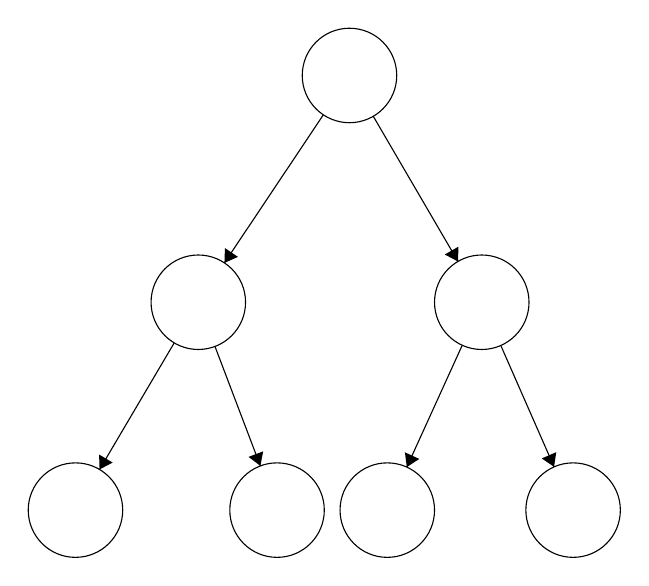
\begin{tikzpicture}[scale=0.2]
\tikzstyle{every node}+=[inner sep=0pt]
\draw [black] (43.1,-8.3) circle (3);
\draw [black] (33.5,-22.7) circle (3);
\draw [black] (51.5,-22.7) circle (3);
\draw [black] (25.7,-35.9) circle (3);
\draw [black] (38.5,-35.9) circle (3);
\draw [black] (45.5,-35.9) circle (3);
\draw [black] (57.3,-35.9) circle (3);
\draw [black] (41.44,-10.8) -- (35.16,-20.2);
\fill [black] (35.16,-20.2) -- (36.02,-19.82) -- (35.19,-19.26);
\draw [black] (44.61,-10.89) -- (49.99,-20.11);
\fill [black] (49.99,-20.11) -- (50.02,-19.17) -- (49.15,-19.67);
\draw [black] (31.97,-25.28) -- (27.23,-33.32);
\fill [black] (27.23,-33.32) -- (28.06,-32.88) -- (27.2,-32.37);
\draw [black] (34.56,-25.51) -- (37.44,-33.09);
\fill [black] (37.44,-33.09) -- (37.62,-32.17) -- (36.69,-32.52);
\draw [black] (50.26,-25.43) -- (46.74,-33.17);
\fill [black] (46.74,-33.17) -- (47.53,-32.65) -- (46.62,-32.23);
\draw [black] (52.71,-25.45) -- (56.09,-33.15);
\fill [black] (56.09,-33.15) -- (56.23,-32.22) -- (55.31,-32.62);
\end{tikzpicture}
\end{center}
Since this is a complete graph we can consider the case where the root is not included in the set, this means that we will consider all possible combinations of independent sets with the children which we know to be $L(n-1)$ and we consider them with the combination with the level below the root node, of which there are 2, thus $L(n-1)^2$. If we include the root node, then the $n-2$ level will be able to form combinations of independent sets with the lowest level in the subtree thus giving us $L(n-2)^4$ since there are 4 grandchildren. Thus this gives us the recursion:
\begin{align*}
L(n) = L(n-1)^2 + L(n-2)^4
\end{align*}
\begin{align*}
\end{align*}



\section*{Problem 2}
\subsection*{Randomized Algorithm}
Divided the vertices into $k$ sets using a fair, random algorithm such as a $k-$-sided die. The probability that an edge corsses between different sets is $\frac{k-1}{k}$ because there are $k$ possible sets for the first vertex to be in and there are $k-1$ possible sets for the second vertex to be in that is different that the set of the first vertex. Thus on average there is expected to be $\frac{k-1}{k}$ edges to cross the cut. Since the most we could have is for all the edges to cross the cut, the random assignment will, on average, be within a factor of $\frac{k}{k-1}$ of optimal.

\subsection*{Local Search Algorithm}
Split the vertices into $k$ sets $S_1,S_2, ..., S_k$. Start with all the verticies in one set. This algorithm will be derived from the MAXCUT algorithm described in class but when swapping a vertex $v$ consider it's placement within each set $S_1, .., S_k$ and swap the vertex to the set that has the greatest improvement on the number of edges that crosses the cut. If swap to multiple sets has equal improvement, pick one of these sets arbitraily to swap the vertex into. Repeat this action until the cut can no longer be improved by a switch.\\

We can count the edges in the cut in the following way: consider any vertex $v \in S_i$. For every vertex $w \in S_j$ where $i \not= j$ that is connected to by an edge, we add $\frac{k}{k-1}$ to a running sum. We do the same for each vertex in the remaning sets $S_1, ... ,S_k \setminus S_i$. Hence the cut C satisfies:
\begin{align*}
C = \frac{k-1}{k} \sum_{i=0}^{k} \bigg( \sum_{v \in S_i}^{} |w:(v,w) \in E, w \not \in S_i| \bigg)
\end{align*}
Since we are using a local search algorithm, at least $\frac{k-1}{k}$ of the edges from any vertex $v$ must lie in a set that $v$ is not in; otherwise, we could switch that vertex to another set and improve the cut. Hence, if vertex $v$ has degree $\delta (v)$, then:
\begin{align*}
C &\geq \frac{k-1}{2k} \bigg( \sum_{i=0}^{k} \frac{\delta (v)}{2} \bigg)\\
&= \frac{k-1}{k} |E|\\
\end{align*}
thus within $\frac{k}{k-1}$ of the optimal.


\section*{Problem 3}
Consider a graph $G$ with maximum clique size $k$. Let $v_1, v_2, ..., v_k$ be the vertices within the clique. Consider graph $GxG$. In $GxG$ there will be $k^2$ verticies $(v_i,v_j)$ such that $v_i, v_j \in \{v_1, ..., v_k\}$. Consider this vertex $(v_i,v_j)$. For any other point $(v_x, v_y) \in \{v_1, ..., v_k\}$ there will exist edge $\{(v_i,v_j),(v_x,v_y)\}$ because $(v_i,v_x)$ and $(v_j,v_y)$ are edges in $G$ because $v_i,v_j,v_x,v_y$ are verticies in the clique in $G$. Thus when considering the $k^2$ vertices in $GxG$ constructed by pairing $v_1, v_2, ..., v_k$ which belong in the $k$-clique of $G$, these $k^2$ vertices form a $k^2$-clique within $GxG$. Therefore the maximum clique size of $GxG$ will be at least $k^2$.\\

The polynimal time algorithm will approximate a maximum clique in a graph within a factor of 2. Let the maximum clique size of $G$ be $k$. The algorithm will approximate the maximum clique size to be within $(\frac{1}{2}k, 2k)$. Consider $GxG$, which we know has maximum clique size of at least $k^2$. The algorithm will approximate the maximum clique size of $GxG$ to be $(\frac{1}{2}k^2, 2k^2)$. We can reduce the construction of $GxG$ utilizing a similar arguement as shown above to show that if the maximum clique size of $GxG$ is shown to be $k^2$ then the maximum clique size of $G$ is $k$. Thus if the maximum clique size of $GxG$ is approximated to $(\frac{1}{2}k^2, 2k^2)$ then this also approximates the maximum clique size of $G$ to be $(\frac{1}{\sqrt{2}}k, \sqrt{2}k)$. A similar arguement can be shown that using graph $(GxG)x(GxG)$ (applying the construction of $GxG$ on two $GxG$ graphs) which approximates the maximum clique size of $G$ to be $(\frac{1}{\sqrt[4]{2}}k, \sqrt[4]{2}k)$. By extension applying the $GxG$ construction $n$ times will approximate the maximum clique size to be within $((\frac{1}{2})^{\frac{1}{2^n}}k, 2^{\frac{1}{2^n}}k)$. To find a polynomial algorithm that approximates the maximum clique size within a factor of $(1+\varepsilon)$ we need to find how many times $n$ that the $GxG$ construction should be applied such that $\frac{1}{2}^{\frac{1}{2^n}}k \geq \frac{1}{1+\varepsilon}k$ and $2^{\frac{1}{2^n}}k \leq (1+\varepsilon)k$.\\

These inequalities can be calculated as follows.
\begin{align*}
\frac{1}{2}^{\frac{1}{2^n}}k &\geq \frac{1}{1+\varepsilon}k\\
\frac{1}{2^n}log(\frac{1}{2}) &\geq -log(1+\varepsilon)\\
\frac{1}{2^n} &\leq \frac{log(1+\varepsilon)}{log2}\\
\frac{1}{2^n} &\leq log_2(1+\varepsilon)\\
-nlog2 &\leq log(log_2(1+\varepsilon))\\
n &\geq - \frac{log(log_2(1+\varepsilon))}{log2}\\
n &\geq -log_2(log_2(1+\varepsilon))\\
\end{align*}
\begin{align*}
2^{\frac{1}{2^n}}k &\leq (1+\varepsilon)k\\
frac{1}{2^n}log2 &\leq log(1+\varepsilon)\\
frac{1}{2^n} &\leq \frac{log(1+\varepsilon)}{log2}\\
frac{1}{2^n} &\leq log_2(1+\varepsilon)\\
-nlog2 &\leq log(log_2(1+\varepsilon))\\
n &\geq -\frac{log(log_2(1+\varepsilon))}{log2}\\
n &\geq -log_2(log_2(1+\varepsilon))\\
\end{align*}

Therefore to find a polynomial time algorihtm for approximating a maximum clique in a graph within a factor of $(1+\varepsilon)$, apply the $GxG$ construction $n$ times such that $n \geq -log_2(log_2(1+\varepsilon))$, use the polynomial time algorithm that approximates to a factor of 2 to approximate the maximum clique within the $GxG$ constructed graph and reducing it to approximate the maximum clique of $G$ within a factor of $(1+\varepsilon)$.
\section*{Problem 4}
\subsection*{Terminate to Stable State}
 Let us label the two machines A and B, where $A$ has a higher load time than $B$. Let the jobs in machine $A$ have run times $r_{a_1}, r_{a_2}, ..., r_{a_i}$ and the jobs in machine $B$ have run times $r_{b_1}, r_{b_2}, ..., r_{b_j}$. Let $r_s$ be time separation between the two machines. The goal is to move a job on machine A with some run time $r_{a_x}$ where $r_{a_x} < r_s$ to machine B,  which will ultimately update $r_s$ to decrease. Let $r_{a_{min}}$ be the minimum job time of a job on $A$. $r_{a_{min}}$ will swap whenever $r_{a_{min}} < r_s$ which implies that stable state will be reached when when $r_{a_{min}} \geq r_s$. Realize that there is a hard cap of what $r_{a_{min}}$ can be and that is $r_{a_{min}} \geq 0$ because run times of a job would never be negative. $r_s$ will decrease with every swap and a swap will always happen when $r_{a_{min}} < r_s$ because the job with run time $r_{a_{min}}$ could be swapped to machine B and then the new minimum run time on machine A, $r'_{a_{min}}$, would be $r'_{a_{min}} \geq r_{a_{min}}$. If $r'_{a_{min}} \geq r_s$ then we will reach stable state, else repeat the process. Since $r_{a_{min}}$ has a hard cap of $r_{a_{min}}\geq 0$, stable state must occur because swaps can occur until $r_s = 0$ because there will not exist an infinite number of jobs such that $r_{a_{min}} < r_s$ will always hold true.

\subsection*{Factor 4/3 of optimal}
To show that the completion time is within a factor of $\frac{4}{3}$ of the optimal, prove by contradition. Consider have two machines $X$ and $Y$ at stable state with overall machine run time of $r_X$ greater than overall run time $r_Y$. Assume for the sake of contradiction. that $r_X > \frac{4}{3} opt$. We determined previously that $opt \geq \frac{r_X+r_Y}{2}$ thus it follows
\begin{align*}
r_X&>\frac{4}{3} opt \geq \frac{4}{3}\bigg(\frac{r_X+r_Y}{2}\bigg)\\
r_X&> \frac{2}{3}(r_X+r_Y)\\
r_X&>2r_Y \\
\end{align*}
The machines are at a stable point, thus that no swapping from $X$ to $Y$ will decrease $r_s$. As described above the job in $X$ with the lowest run time $r_{x_{min}}$ such that $r_{x_{min}} \geq r_s$. Because $r_X>2r_Y$ then the time seperation between the two machines must be greater that $r_Y$ or $r_s>r_Y$. Thus $r_{x_{min}} > r_Y$. This would only exist in stable state if $X$ only contain the largest time consuming job. From assignment 3, we proved that if one machine has the largest job and that job is larger than all the other jobs summed together on the other machine, then that is the most optimal configuration. Thus $r_X = opt$. This contradicts the assumption that $X>\frac{4}{3}opt$. This implies that $X \leq \frac{4}{3}opt$
\end{document}
